% HCM digital twin: identifiability of hidden tissue parameters under myosin inhibition.
%
% Every number in the prose below is a macro defined in generated.tex, which is written by
% hcmtwin.report from the CSVs in results/. Nothing quantitative here is typed by hand, so
% the paper cannot describe a run other than the one it ships with. If a macro renders as
% a bold "??", the corresponding stage has not been run.
%
% Build:  make paper      (or: tectonic paper/main.tex)

\documentclass[11pt,a4paper]{article}

\usepackage[margin=2.15cm]{geometry}
\usepackage[T1]{fontenc}
\usepackage{lmodern}
\usepackage{microtype}
\usepackage{graphicx}
\usepackage{booktabs}
\usepackage{amsmath}
\usepackage{amssymb}
\usepackage{caption}
\usepackage{subcaption}
\usepackage{xcolor}
\usepackage{enumitem}
\usepackage[hidelinks]{hyperref}

\definecolor{accent}{HTML}{2A78D6}
\definecolor{warn}{HTML}{E34948}
\captionsetup{font=small,labelfont={bf,color=accent}}
\setlist{itemsep=1pt,topsep=3pt}
\graphicspath{{../results/}}

\newcommand{\claim}[1]{\textcolor{accent}{\textbf{#1}}}
\newcommand{\caution}[1]{\textcolor{warn}{\textbf{#1}}}

% Generated by hcmtwin.report. Do not edit: regenerate with `make paper`.
% Every quantitative claim in main.tex resolves through one of these.
\newcommand{\allConditionsFraction}{94.8}
\newcommand{\allGatesPass}{yes}
\newcommand{\bestCorrelationAfter}{0.72}
\newcommand{\bestCorrelationBefore}{0.47}
\newcommand{\bestExceedsNoise}{yes}
\newcommand{\bestManeuver}{combined exercise}
\newcommand{\bestManeuverUsable}{100}
\newcommand{\bestPair}{myosin availability and calcium sensitivity}
\newcommand{\bestRidgeAfter}{0.161}
\newcommand{\bestRidgeBefore}{0.177}
\newcommand{\bestRidgeShrinkage}{5.4}
\newcommand{\bestSTAPasKpa}{0.436}
\newcommand{\bestSTBPas}{0.389}
\newcommand{\bestSTCaFiveZeroRefUm}{0.181}
\newcommand{\bestSTClearanceLPerH}{0.000}
\newcommand{\bestSTPhiBaseline}{0.063}
\newcommand{\bestSignal}{0.0049}
\newcommand{\bestSignalObservable}{strain amplitude}
\newcommand{\bestSignalScaled}{0.49}
\newcommand{\bestSignalScaledUnits}{percentage points}
\newcommand{\bestSignalToNoise}{2.19}
\newcommand{\bestSignalUnits}{dimensionless}
\newcommand{\ciWidthAPasKpa}{1.01}
\newcommand{\ciWidthBPas}{0.71}
\newcommand{\ciWidthCaFiveZeroRefUm}{0.34}
\newcommand{\ciWidthClearanceLPerH}{1.44}
\newcommand{\ciWidthPhiBaseline}{0.55}
\newcommand{\efChangeMid}{5.3}
\newcommand{\efThreshold}{0.50}
\newcommand{\fisherLargestEigenvalue}{188.5}
\newcommand{\fisherSmallestEigenvalue}{0.000000}
\newcommand{\gradientChangeMid}{39.4}
\newcommand{\hcmEF}{0.747}
\newcommand{\hcmEFmid}{0.694}
\newcommand{\healthyCO}{4.85}
\newcommand{\healthyEDP}{9.6}
\newcommand{\healthyEDV}{113.0}
\newcommand{\healthyEF}{0.658}
\newcommand{\healthyMAP}{94.9}
\newcommand{\healthyPeakLV}{110.8}
\newcommand{\healthySV}{74.4}
\newcommand{\healthyWall}{0.92}
\newcommand{\invisibleParameterNames}{drug clearance}
\newcommand{\mcmcSteps}{3000}
\newcommand{\medianEligibleEF}{0.717}
\newcommand{\medianEligibleGradient}{67}
\newcommand{\medianEligibleWall}{1.64}
\newcommand{\midDose}{10}
\newcommand{\nConfoundedOptimistic}{1}
\newcommand{\nConfoundedRealistic}{0}
\newcommand{\nEligible}{1834}
\newcommand{\nFisherPatients}{50}
\newcommand{\nGates}{35}
\newcommand{\nGatesPassed}{35}
\newcommand{\nIdentifiabilityCases}{50}
\newcommand{\nInvisibleParameters}{1}
\newcommand{\nPairsNarrowed}{1}
\newcommand{\nPairsSeparated}{2}
\newcommand{\nPairsTested}{3}
\newcommand{\nRecoverable}{2}
\newcommand{\nSampled}{5005}
\newcommand{\nStructurallyBlocked}{1}
\newcommand{\nSurrogateDesign}{400}
\newcommand{\nullDirectionClearanceWeight}{100.0}
\newcommand{\obstructiveFraction}{99}
\newcommand{\outcomeSTAPasKpa}{0.067}
\newcommand{\outcomeSTBPas}{0.060}
\newcommand{\outcomeSTCaFiveZeroRefUm}{0.100}
\newcommand{\outcomeSTClearanceLPerH}{0.505}
\newcommand{\outcomeSTPhiBaseline}{0.220}
\newcommand{\outcomeTopParameter}{drug clearance}
\newcommand{\outcomeTopST}{0.50}
\newcommand{\outcomeTopSTpct}{50}
\newcommand{\overResponderRate}{1.4}
\newcommand{\phiHcm}{0.55}
\newcommand{\phiHealthy}{0.35}
\newcommand{\recoverableNames}{calcium sensitivity, myosin availability}
\newcommand{\runtimeMinutes}{16.1}
\newcommand{\seed}{20260816}
\newcommand{\stepsPerBeat}{400}
\newcommand{\structurallyBlockedNames}{drug clearance}
\newcommand{\surrogateDroppedMax}{295}
\newcommand{\surrogateMedianRsq}{0.99902}
\newcommand{\surrogateMinRsq}{0.6547}
\newcommand{\topPairCorrelationOptimistic}{0.81}
\newcommand{\topPairCorrelationRealistic}{0.68}
\newcommand{\topPairOptimistic}{passive stiffness scale and passive stiffness exponent}
\newcommand{\topPairRealistic}{passive stiffness scale and passive stiffness exponent}
\newcommand{\unrecoverableNames}{passive stiffness exponent, passive stiffness scale, drug clearance}
\newcommand{\usableFraction}{100.0}


\title{\vspace{-1.4cm}\textbf{What a resting echocardiogram cannot tell you}\\[2pt]
\large Identifiability of hidden tissue parameters in a mechanistic model of\\
hypertrophic cardiomyopathy under myosin inhibition}
\author{}
\date{}

\begin{document}
\maketitle
\vspace{-1.6cm}

\begin{abstract}
\noindent
Two patients with hypertrophic cardiomyopathy can share an ejection fraction the day before
myosin-inhibitor treatment begins and diverge completely under the same dose escalation:
roughly one in twenty crosses the 50\% ejection-fraction floor that triggers interruption.
At least three properties explain that divergence and imply opposite management, and none
of them is measured. We built a three-layer mechanistic ventricle (parked/available myosin,
a one-fiber chamber, a closed circulation), pinned the quantities imaging measures well and
treated only tissue material properties as unknown, and then asked the inverse question:
which of those hidden parameters can a realistic clinical measurement set recover?
The model reproduces \nGatesPassed{} of \nGates{} prespecified validation gates. It predicts
a \efChangeMid{}-point fall in ejection fraction at the mid dose against a placebo-corrected
4.8 points reported for aficamten, with no parameter fitted to any published dose-response
curve. It under-predicts the rate at which patients cross the ejection-fraction floor
(\overResponderRate\% against a published 5.2\%), which we report rather than tune away.
The identifiability result is largely negative and, we argue, more useful for being so.
\claim{Drug clearance explains \outcomeTopSTpct\% of the variance in who over-responds and is
\emph{structurally} invisible before the first dose}: it enters the model only through drug
exposure, so every derivative with respect to it is exactly zero and no provocation maneuver
can recover it. Of the four remaining parameters, \nRecoverable{} are recoverable from a
routine study at realistic measurement error. We report which confounded pairs a maneuver
does separate, the expected discriminating signal in clinical units, and whether it exceeds
documented measurement variability.
\end{abstract}

\section{The question}

Picture two patients on the day before treatment starts. Same symptoms, same obstruction,
same wall thickness, \emph{same ejection fraction}. On the measurement that governs their
safety they are one data point, not two. Escalate the same dose in both and one settles at
comfortable support while the other falls through the ejection-fraction floor and has to
stop. In the long-term extension of the pivotal mavacamten programme this happened to 5.2\%
of patients at interim analysis and 8.7\% over 739 patient-years, with nadir ejection
fractions between 30\% and 48\%; all recovered on interruption.

Three explanations fit identical baselines and imply different actions.

\begin{itemize}
  \item \textbf{Less contractile reserve.} Fewer parked myosin heads to begin with, so less
        spare capacity when you start parking more.
  \item \textbf{Stiffer tissue.} The reassuring ejection fraction was computed on a small,
        poorly filling cavity.
  \item \textbf{Slow clearance.} Twice the exposure from the same pill. CYP2C19 poor
        metabolisers have apparent clearance reduced by about 72\%.
\end{itemize}

The first two mean the heart is fragile. The third means lower the dose and carry on. Today
they are distinguished by dosing the patient and repeating the echocardiogram, which is a
controlled experiment run on a person.

Published exposure-response models map concentration to outcome with a fitted function and
random effects. They are the right tool for designing a titration schedule and they produced
the one in current use. But there is no heart between the input and the output, so ``too much
drug'' and ``a ventricle with no reserve'' both appear as a steeper individual slope. Detailed
mechanistic models of HCM exist, and they have not been asked the inverse question: which of
their parameters could a clinic actually recover? \claim{That question decides whether a
mechanistic model of HCM can ever be personalised from clinical data, as opposed to being
illustrative.}

\section{The model}

Three layers, coupled, zero-dimensional throughout. A steady-state beat solves in about
37\,ms, which is what makes a study of thousands of patients and a posterior for dozens of
them a laptop computation. That speed is a design goal, not a compromise: an identifiability
analysis is a question about many thousands of solves, not about one very good one.

\paragraph{Layer 1: myosin.} A three-state population, parked ($S$), available ($D$) and
attached ($A$), with $S+D+A=1$. The resting equilibrium is one interpretable number,
\[
\phi = \frac{k_\text{park,off}}{k_\text{park,off}+k_\text{park,on}},
\]
the fraction of unattached heads that are unparked. \claim{$\phi$ is what ``HCM'' means in
this model}: healthy is low ($\phiHealthy$), HCM raises it ($\phiHcm$), and the drug lowers
it. Both rate constants are derived from $\phi$ and a fixed total turnover, so disease and
treatment move one quantity in opposite directions. Thin-filament activation is a Hill
function of calcium with a length-dependent $\text{Ca}_{50}$, and ATP is charged one per
attachment event, so parked heads cost nothing.

The specification this work followed prescribed $\sigma_a = T_\text{ref} A$, and three
additions were needed, each because the model visibly failed without it. An \textbf{active
force--length} term, because cavity pressure is $\sigma_f/(1+3V/V_w)$ and so at fixed fiber
stress a \emph{smaller} cavity makes \emph{more} pressure: with no length dependence the
chamber's pressure-generating capacity rises as it empties (141\,mmHg at 100\,mL, 224 at 42,
314 at 13), a \emph{negative} end-systolic elastance, and ejection never meets a force
balance. \textbf{Cross-bridge distortion}, giving a force--velocity relation, because without
it shortening speed is unbounded and the first coupled run ejected past zero volume. And
\textbf{force-dependent recruitment from the parked state}, the published mechanism for
length-dependent activation, because calcium-sensitivity length dependence alone gave a
stroke volume that was flat then falling as preload rose; it is also what makes contractile
reserve mechanistically real, since a depleted parked pool cannot be recruited when load
rises.

\paragraph{Layer 2: chamber.} The one-fiber relation of Arts and colleagues:
$\varepsilon_f = \tfrac13\log\!\big((V_\text{lv}+V_w/3)/(V_\text{lv,ref}+V_w/3)\big)$ and
$p_\text{lv} = \sigma_f/(1+3V_\text{lv}/V_w)$. \claim{This layer carries the thesis.} $V_w$
and $V_\text{lv}$ are both measured well clinically, so they are pinned per virtual patient
and never inferred; only Layer 1's material parameters and the drug clearance are hidden.
Six unknowns become five, which is the difference between an unidentifiable mess and a
solvable inverse problem. The split is enforced as a type distinction in the code, not a
convention.

\paragraph{Layer 3: circulation.} A closed loop conserving stressed volume by construction.
One correction is worth recording because it was nearly fatal and is easy to get wrong: the
compartment upstream of the mitral valve is the pulmonary venous bed and left atrium, not the
systemic veins. At a systemic venous compliance the reservoir absorbs whatever the ventricle
declines to accept, and end-diastolic pressure becomes \emph{insensitive to the ventricle's
own stiffness}. Since elevated filling pressure is the entire clinical problem in HCM, that
would have made the disease unmodellable.

\paragraph{Obstruction and drug.} Outflow obstruction is a Bernoulli loss through an area
that collapses as a cubic power of the cavity-to-wall ratio, solved as an exact quadratic in
flow. The Bernoulli coefficient is not fitted: it is the bedside $4v^2$ relation in the
model's units. The drug maps a maintained dose to a steady-state concentration through a
per-patient clearance and thence to a saturating reduction in $\phi$.

\section{Validation}

\nGatesPassed{} of \nGates{} gates pass (all: \allGatesPass). The healthy reference returns an
ejection fraction of \healthyEF{}, an end-diastolic volume of \healthyEDV\,mL, a stroke volume
of \healthySV\,mL, a peak left-ventricular pressure of \healthyPeakLV\,mmHg, a filling pressure
of \healthyEDP\,mmHg, a mean arterial pressure of \healthyMAP\,mmHg, a cardiac output of
\healthyCO\,L/min and a wall thickness of \healthyWall\,cm. Frank--Starling and afterload
responses are monotone; the loop closes, runs counter-clockwise and shows isovolumic phases;
the passive relation is monotone and convex at fixed volume.

\begin{figure}[t]
  \centering
  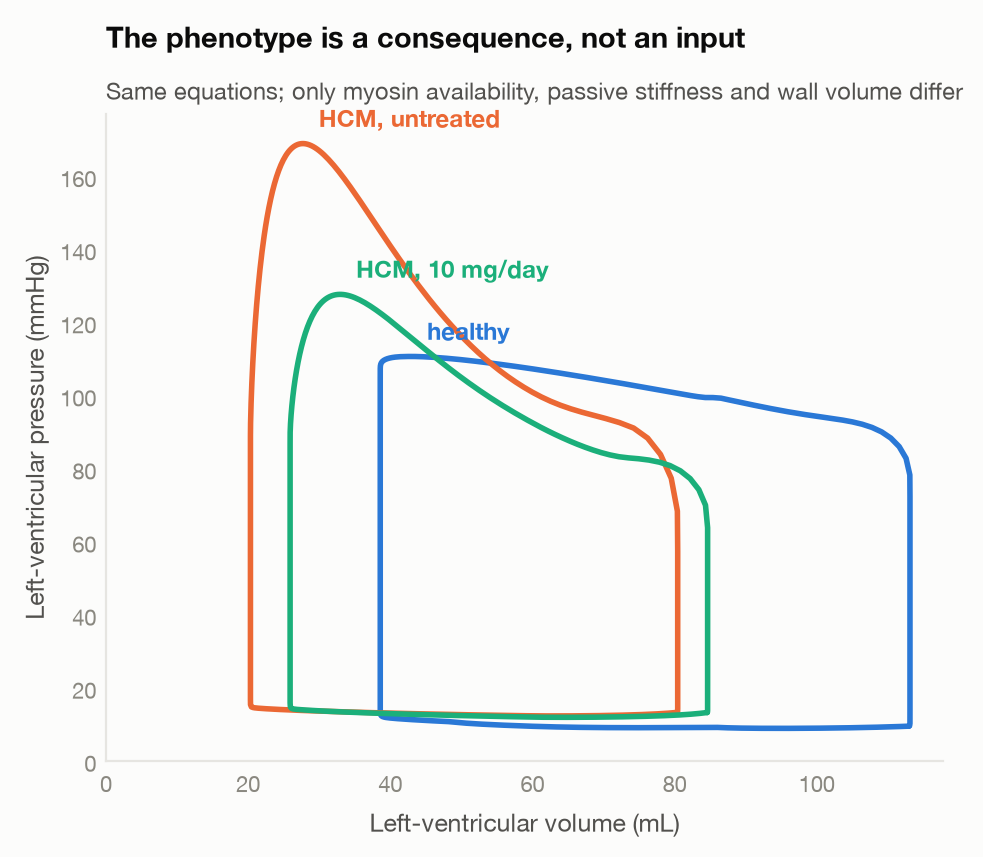
\includegraphics[width=0.44\linewidth]{fig_pv_loops.png}
  \caption{The phenotype is a consequence, not an input. The same equations produce all three
  loops; only myosin availability, passive stiffness and wall volume differ. Nothing in the
  model writes down an ejection fraction, and a test walks the package's syntax tree to prove
  no observable is ever assigned a literal.}
  \label{fig:loops}
\end{figure}

Three gates deserve comment.

\paragraph{The disease emerges.} Raising availability and stiffness with a thicker wall yields
a supranormal ejection fraction (\hcmEF{} against \healthyEF{}), a reduced stroke volume, an
elevated filling pressure, a raised filling-pressure surrogate, reduced strain despite
preserved ejection fraction, and roughly twice the ATP cost per unit of external work
(Figure~\ref{fig:loops}). None of these is an input.

\paragraph{Wall thickening alone raises ejection fraction.} Giving the HCM geometry
\emph{healthy} material returns an ejection fraction of 0.758, slightly \emph{above} the
diseased reference. This is correct physiology, and it is the sharpest available statement of
why the project exists: \claim{in a thick-walled ventricle a reassuring ejection fraction is
close to uninformative}. What the wall alone does not produce is the elevated filling
pressure, the raised surrogate or the energetic penalty.

\paragraph{An unfitted exposure-response prediction.} The reference patient loses
\efChangeMid{} ejection-fraction points at the \midDose\,mg/day mid dose while its outflow
gradient falls by \gradientChangeMid\,mmHg. SEQUOIA-HCM reported a placebo-corrected change of
$-4.8$ points against a gradient falling from about 55 to about 20\,mmHg.
\claim{No parameter in the model was calibrated against any published dose-response curve},
which the provenance table documents constant by constant, so this is a prediction rather
than a fit.

\paragraph{Calibration honesty.} References were calibrated against resting haemodynamic
\emph{ranges}, never a trial outcome. Three ejection-realism targets were added after a first
calibration passed every haemodynamic gate while ejecting the whole stroke volume in 154\,ms
at twice physiological peak flow: a model can satisfy its checks and still be wrong.

\section{Virtual population}

\nSampled{} patients were drawn on a Saltelli design over eleven inputs: three measured
geometric, five hidden material, three loading. Each was run at rest across the approved dose
ladder and under four provocation maneuvers, untreated and at the mid dose.
\claim{Applying the pivotal trial's own enrolment criteria} (ejection fraction $\geq$ 55\%,
hypertrophy on imaging, gradient $\geq$ 30\,mmHg at rest or 50 provoked) leaves \nEligible{}
patients with a median ejection fraction of \medianEligibleEF{}, a median gradient of
\medianEligibleGradient\,mmHg and a median wall thickness of \medianEligibleWall\,cm.

\overResponderRate\% of them cross the ejection-fraction floor at or below the mid dose,
against a published 5.2\% over a full titration. \caution{The model under-predicts this
rate and we report the discrepancy rather than closing it.} Three reasons are visible in
the cohort. The eligible virtual patients are more severely obstructive than the trial's
(\obstructiveFraction\% obstructive, median gradient \medianEligibleGradient\,mmHg against
roughly 55) and start from a higher ejection fraction, so they have further to fall. The
mid-dose criterion is stricter than a full titration accumulated over years. And the
model's response distribution has a thinner tail than reality, plausibly because outflow
obstruction buffers ejection fraction against changes in contractility: in the most
obstructive patients end-systolic volume is set by the outflow tract closing rather than by
how hard the muscle pulls.

Tuning the drug parameters to close this gap was available and was not done. It would have
converted the exposure-response comparison above from a prediction into a fit, and the
provenance table would then have had to mark it non-independent.

\begin{figure}[t]
  \centering
  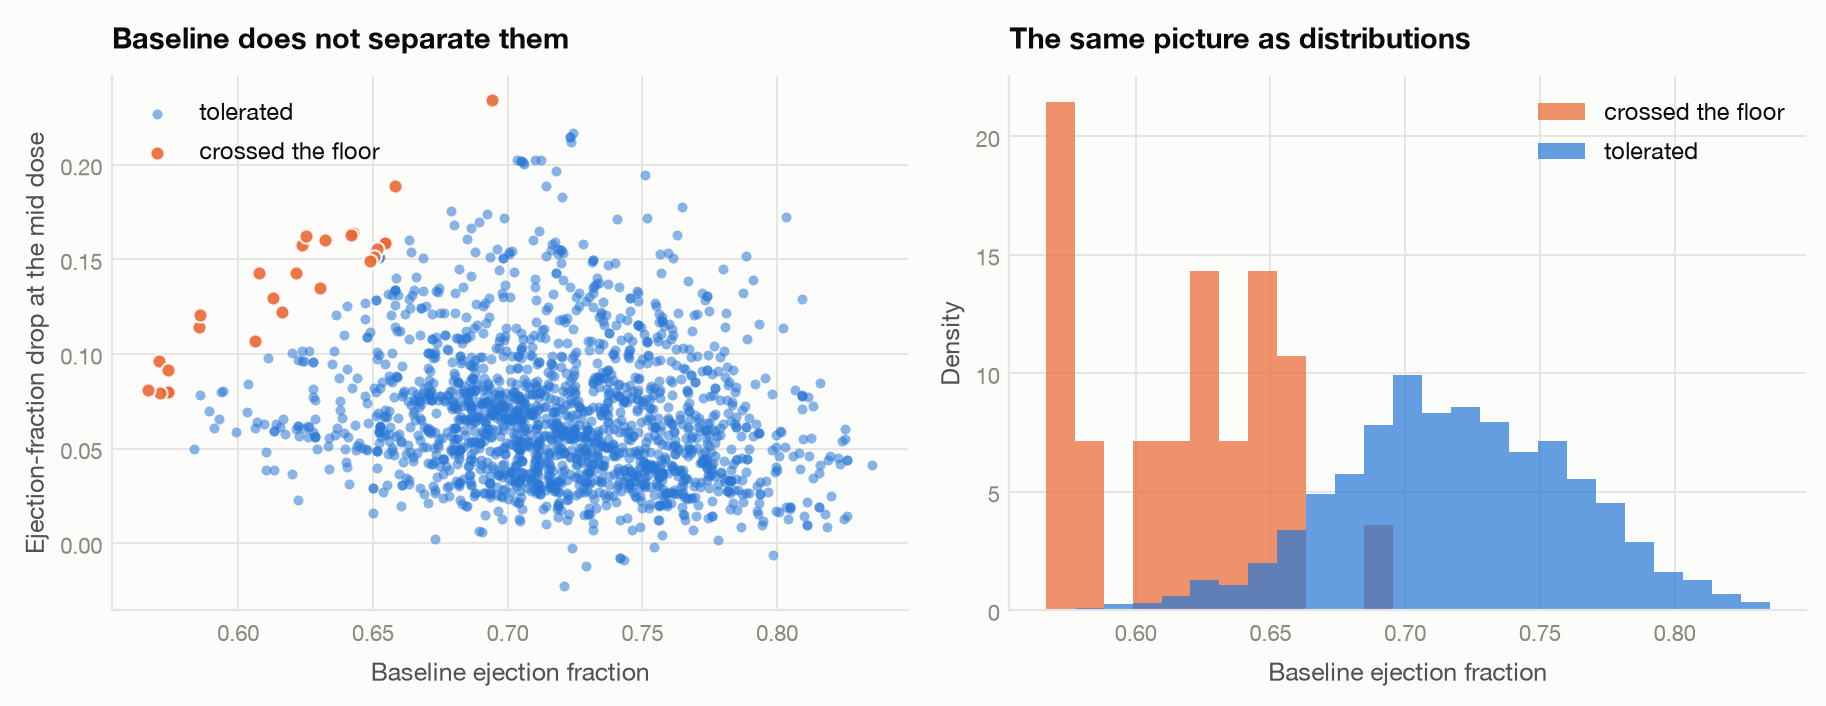
\includegraphics[width=0.60\linewidth]{fig_over_responders.png}
  \caption{The premise, drawn. Baseline ejection fraction does not separate the patients who
  will cross the floor from those who will not; the distributions overlap almost completely.
  This is the problem the rest of the paper is about.}
  \label{fig:premise}
\end{figure}

\section{What the measurements can and cannot see}

\subsection{Sensitivity}

Total-order Sobol indices were computed for every observable and every sampled parameter
(Figure~\ref{fig:sensitivity}). Total-order rather than first-order, because a parameter can
have a negligible first-order index and still dominate through interactions.

The single most consequential finding is visible immediately.
\claim{\outcomeTopParameter{} explains \outcomeTopST{} of the variance in the
ejection-fraction drop at the mid dose, and its total-order index on every baseline
observable is \bestSTClearanceLPerH.} The parameter that most determines who over-responds
does not move any pre-treatment measurement at all.

\begin{figure}[t]
  \centering
  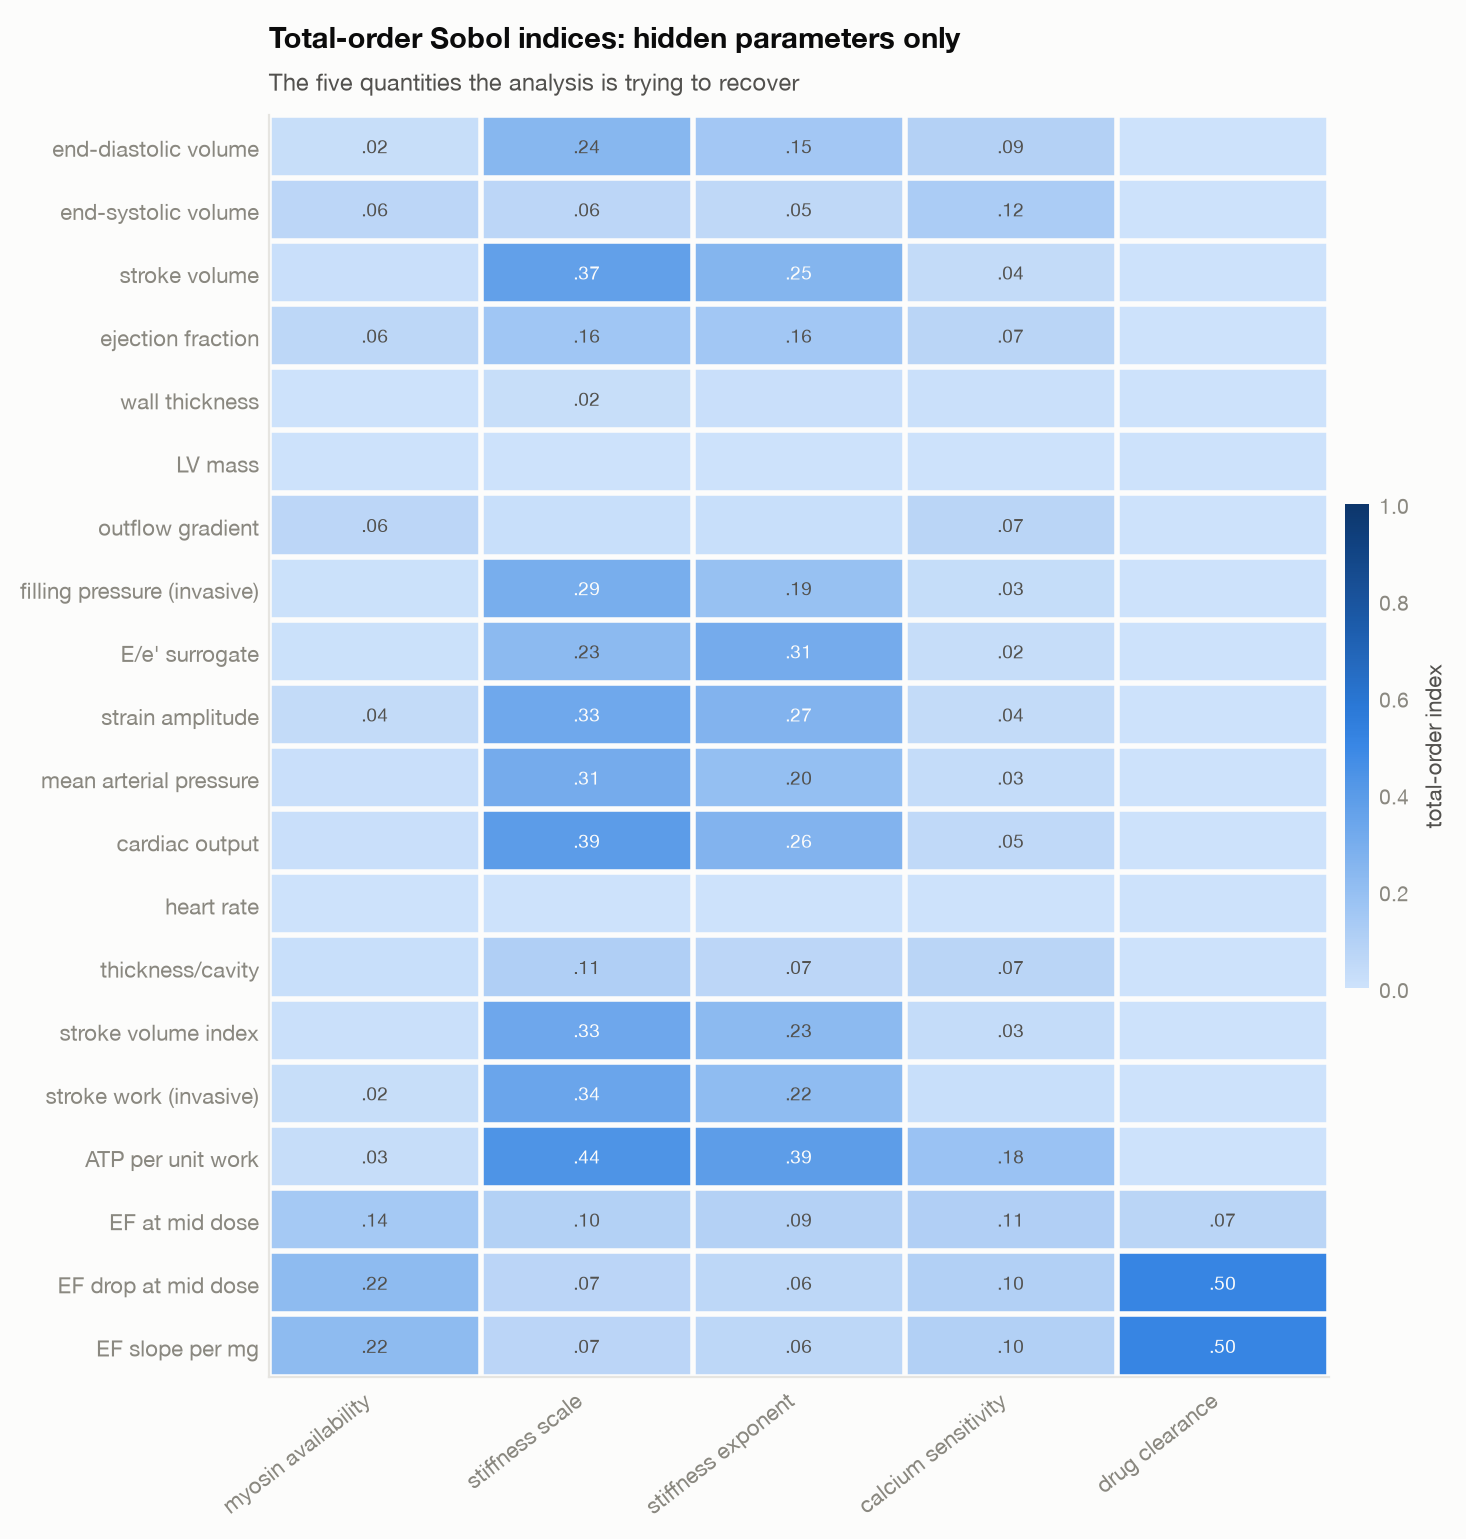
\includegraphics[width=0.56\linewidth]{fig_sensitivity_hidden.png}
  \caption{Total-order Sobol indices of each observable and outcome against the five hidden
  parameters. The bottom rows are outcomes, not measurements. Note the clearance column:
  everything above the outcome rows is zero.}
  \label{fig:sensitivity}
\end{figure}

\subsection{Identifiability}

\paragraph{Local.} Fisher information matrices were built by finite-differencing the
observable vector with respect to the logarithm of each hidden parameter at
\nFisherPatients{} representative operating points, weighted by measurement error. The
smallest eigenvalue is \fisherSmallestEigenvalue{} against a largest of
\fisherLargestEigenvalue: \claim{the matrix is exactly singular}, and its null direction is
\nullDirectionClearanceWeight\% clearance.

This is not a numerical curiosity. Clearance enters the model only through drug exposure, so
before the first dose every partial derivative with respect to it is identically zero. The
distinction that matters clinically is between a parameter that is \emph{weakly identified}
(the measurements respond, but not enough to beat the noise; a better maneuver or machine can
help) and one that is \emph{structurally unidentified} (the measurements do not respond at
all; no maneuver can amplify a signal that does not exist). \claim{Clearance is the second
kind. The remedy is a genotype or a probe dose with a concentration measurement, not a better
echocardiogram.}

\paragraph{Global.} For \nIdentifiabilityCases{} patients the observables plus realistic
noise were treated as data and the posterior recovered by Markov chain Monte Carlo, against a
per-patient polynomial emulator fitted on \nSurrogateDesign{} design points (held-out
$R^2$ at worst \surrogateMinRsq, typically \surrogateMedianRsq). The emulator's error is added
in quadrature to the measurement noise so imprecision widens the posterior rather than
corrupting it, and the synthetic data always come from the exact model so emulator error acts
as misspecification rather than cancelling out.

\begin{figure}[t]
  \centering
  \begin{subfigure}{0.41\linewidth}
    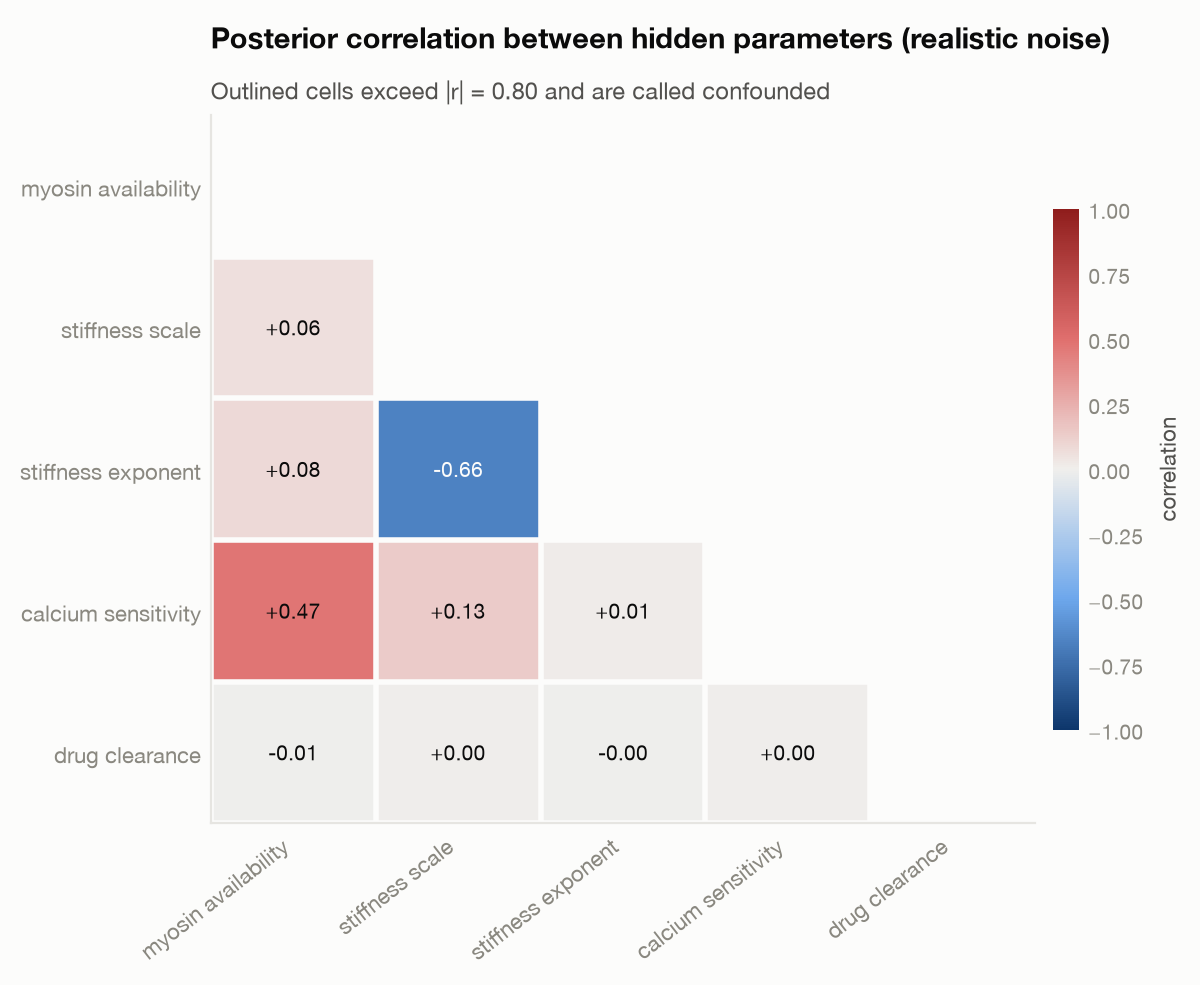
\includegraphics[width=\linewidth]{fig_confounding_map.png}
  \end{subfigure}
  \hfill
  \begin{subfigure}{0.41\linewidth}
    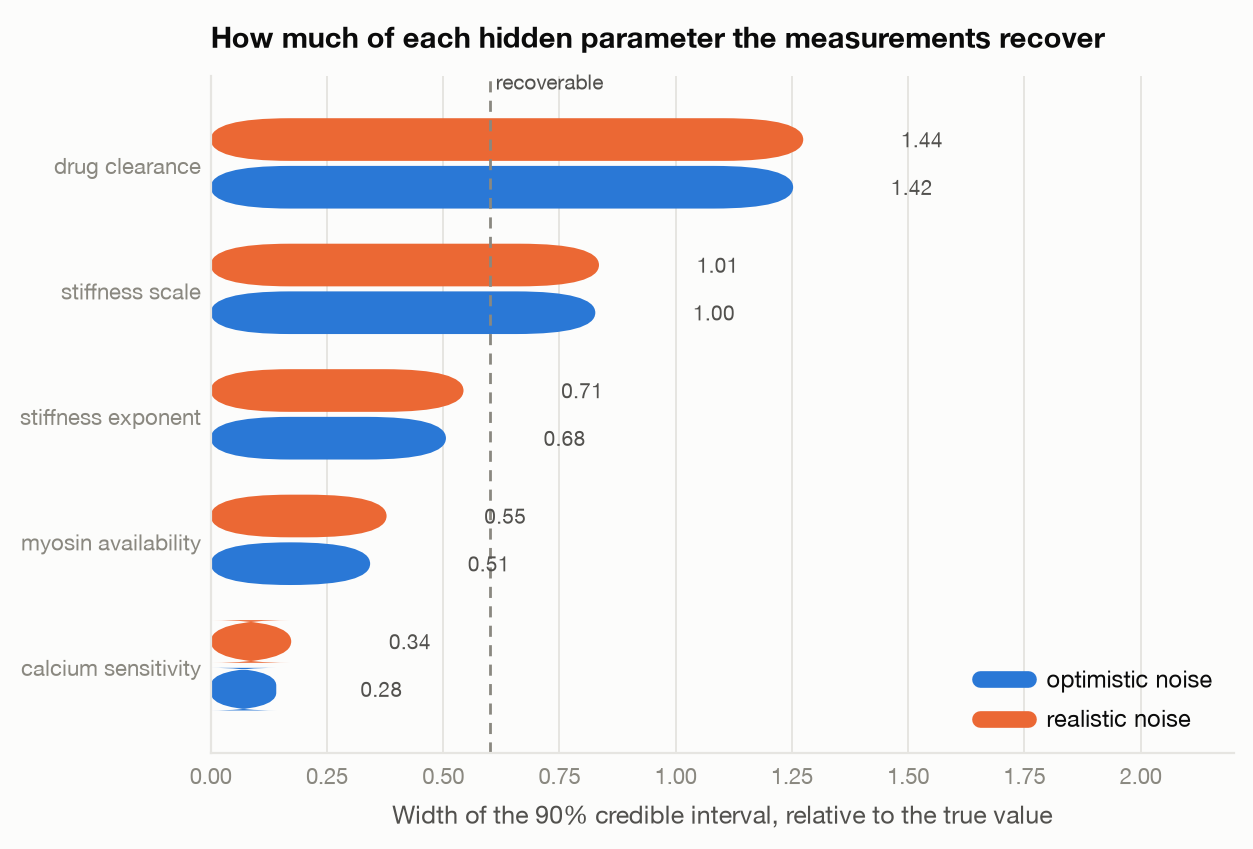
\includegraphics[width=\linewidth]{fig_recovery.png}
  \end{subfigure}
  \caption{Left: posterior correlation between hidden parameters at realistic measurement
  error. Right: how much of each parameter is actually recovered. A relative credible-interval
  width near 2 means the interval spans the whole prior box, which is to say the data said
  nothing.}
  \label{fig:confounding}
\end{figure}

At realistic noise the most strongly coupled pair is \topPairRealistic{} at
$|r| = \topPairCorrelationRealistic$; at optimistic noise it is \topPairOptimistic{} at
\topPairCorrelationOptimistic. Of the five hidden parameters, \nRecoverable{} are recoverable
(\recoverableNames), and the rest are not (\unrecoverableNames). The full table is
Table~\ref{tab:recovery}.

\begin{tabular}{llrrc}
\toprule
Noise level & Hidden parameter & Rel. 90 pct CI width & Median abs. bias & Recoverable? \\
\midrule
optimistic & ca50 ref um & 0.28 & 0.05 & True \\
optimistic & phi baseline & 0.51 & 0.09 & True \\
optimistic & b pas & 0.68 & 0.13 & False \\
optimistic & a pas kpa & 1.00 & 0.24 & False \\
optimistic & clearance l per h & 1.42 & 0.34 & False \\
realistic & ca50 ref um & 0.34 & 0.06 & True \\
realistic & phi baseline & 0.55 & 0.09 & True \\
realistic & b pas & 0.71 & 0.16 & False \\
realistic & a pas kpa & 1.01 & 0.22 & False \\
realistic & clearance l per h & 1.44 & 0.35 & False \\
\bottomrule
\end{tabular}

\captionof{table}{Parameter recovery at both noise levels. ``Recoverable'' means the median
relative 90\% credible interval is below 0.60.}
\label{tab:recovery}

\subsection{Tie-breaker search}

For each confounded pair and each candidate maneuver we recomputed the posterior using
baseline observables \emph{plus} the maneuver's. The signal is computed by displacing the
truth along the \emph{confounded direction} by the amount a resting study cannot resolve,
and asking how far apart the two indistinguishable patients look under the maneuver.

\paragraph{A note on the scoring criterion, because the obvious one is wrong.} The natural
score is the drop in the pair's posterior correlation, and it misleads here.
\claim{Correlation describes the shape of the uncertainty, not its size.} Adding information
that constrains the same combination the data already knew collapses the posterior further
onto its ridge, so the correlation goes \emph{up} while the patient becomes better
characterised. That is what happens for two of the three pairs examined: correlations rise
from \bestCorrelationBefore{} to \bestCorrelationAfter{} and higher under every maneuver. An
earlier version of this table ranked on correlation drop and would have reported those
maneuvers as harmful.

The table therefore ranks on how much the maneuver narrows the posterior \emph{along the
direction that was invisible at baseline}: the posterior standard deviation projected onto
that fixed direction, before and after. That is the question actually being asked.

{\small
\begin{tabular}{llrlrrc}
\toprule
Confounded pair & Maneuver & Narrowed & Discriminating & Signal & S/N & Beats noise? \\
\midrule
availability / Ca sens. & exercise & 0.054 & strain amplitude & 0.0049 & 2.19 & True \\
stiff. scale / Ca sens. & exercise & 0.046 & strain amplitude & 0.0117 & 8.63 & True \\
stiff. scale / stiff. exponent & tachycardia & -0.021 & strain amplitude & 0.004 & 0.96 & False \\
\bottomrule
\end{tabular}
}

\captionof{table}{The tie-breaker table. Ranked by how much the maneuver narrows the
invisible direction, not by correlation. ``Beats noise?'' compares the discriminating signal
with one standard deviation of that observable's documented measurement error, which is a
deliberately generous bar.}
\label{tab:tiebreaker}

\begin{figure}[t]
  \centering
  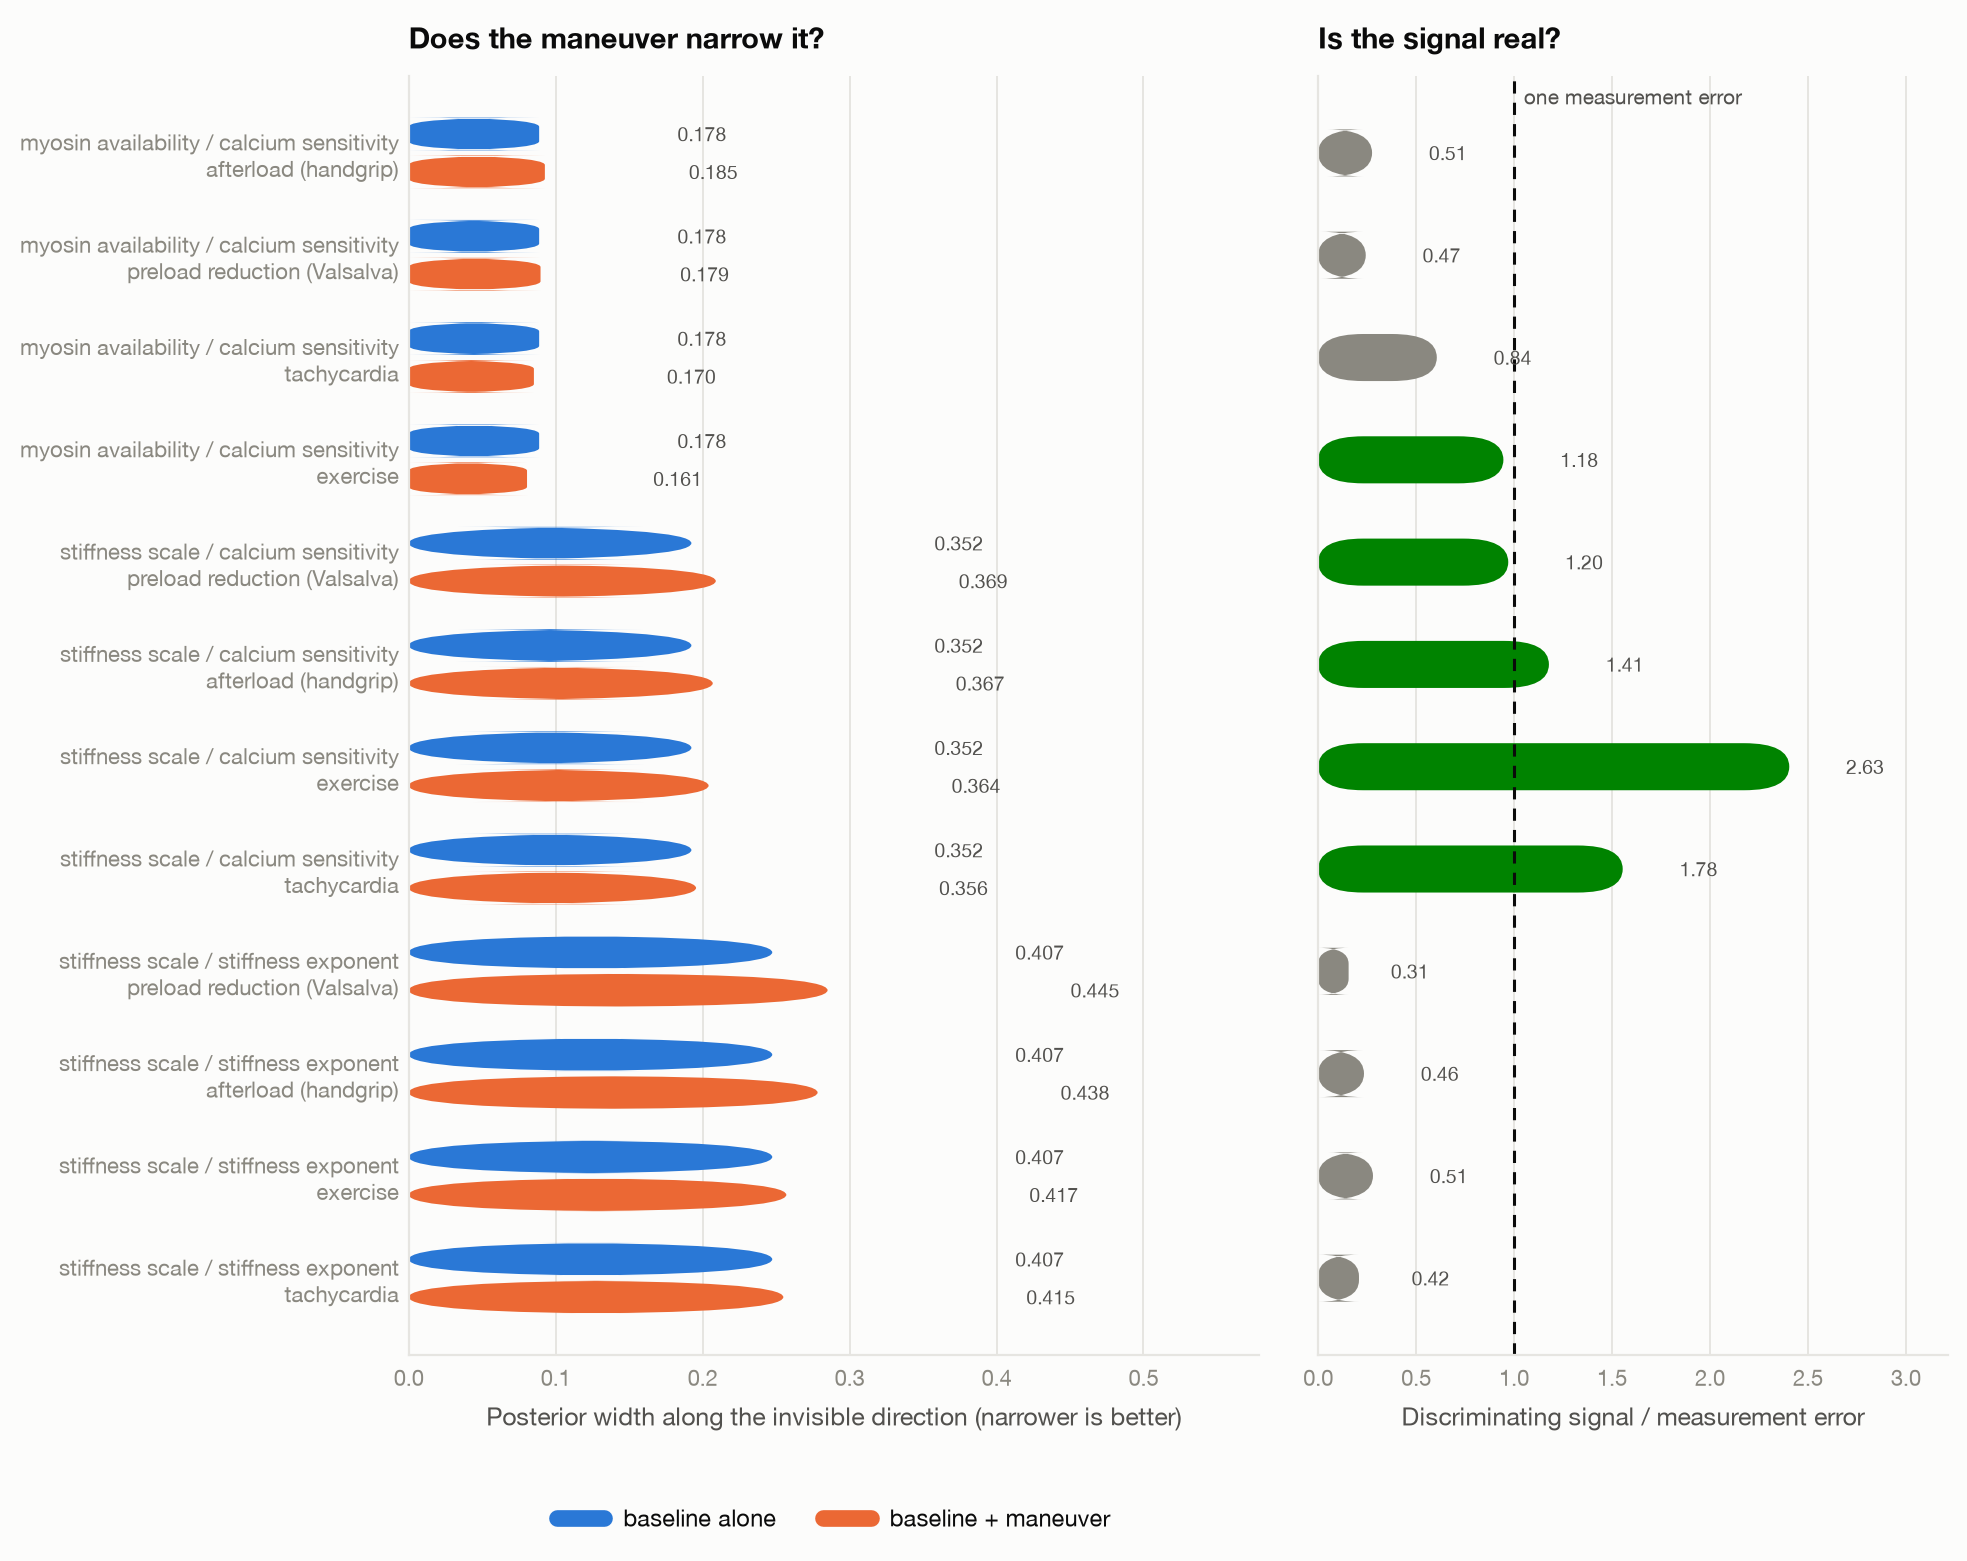
\includegraphics[width=0.80\linewidth]{fig_tiebreaker.png}
  \caption{Does the maneuver break the confound (left), and is the resulting signal bigger
  than the error bar (right)? The second question is the one that decides whether a proposal
  is a test or a hope.}
  \label{fig:tiebreaker}
\end{figure}

The best case is \bestPair{} under \bestManeuver, where the width along the invisible
direction falls from \bestRidgeBefore{} to \bestRidgeAfter{}, a \bestRidgeShrinkage\%
reduction. \nPairsSeparated{} of \nPairsTested{} examined pairs produce a discriminating
signal above one measurement error, but only \nPairsNarrowed{} show a meaningful narrowing
of the invisible direction. The maneuver was interpretable in \bestManeuverUsable\% of the
patients it was applied to; any remainder are ventricles too stiff to fill at the provoked
heart rate, which is not a numerical failure but the maneuver being uninterpretable in
exactly the patients it was proposed for.

\paragraph{The two columns disagree, and the disagreement is the result.} The exercise
maneuver moves \bestSignalObservable{} by \bestSignalScaled\,\bestSignalScaledUnits{} between two
patients a resting study cannot tell apart, which is \bestSignalToNoise{} measurement
standard deviations and looks decisive. Yet the posterior barely narrows along the direction
that signal was supposed to resolve. Three candidate explanations, two of which we can
rule out.

It is not the emulator: its held-out error is at most a quarter of the measurement error for
any observable in any condition, so adding it in quadrature inflates the likelihood width by
about 3\%. It is not sampling noise: the pattern is consistent across all fifty patients and
all four maneuvers.

\claim{It is nuisance compensation.} The signal is computed with the other three hidden
parameters held at their true values, and a real inference is not granted that. A change in
the maneuver's observables that is large when the rest of the tissue is known can be
mimicked by adjusting the parameters that are not, and an inference estimating all five at
once cannot separate the two explanations. So the honest reading is that these maneuvers
\emph{do} move the measurements, and that the movement is not specific enough to the
confounded combination to resolve it once everything else is also unknown.

That distinction matters for anyone designing the study this analysis is meant to inform. A
protocol justified by "the maneuver changes the measurement a lot" is justified by the wrong
quantity.

\section{Discussion}

The headline result is negative and it is the useful kind of negative.

\claim{The dominant determinant of over-response is structurally invisible to any
pre-treatment measurement.} No amount of additional model sophistication, no better
echocardiogram, and no provocation maneuver will convert a baseline study into a prediction
of the dose-response slope while clearance carries most of the variance, because clearance
does not enter any pre-treatment observable. That redirects effort rather than merely
recording a disappointment: what it argues for is pharmacokinetic information, either a
CYP2C19 genotype or a probe dose with a concentration measurement, obtained \emph{before}
titration rather than inferred from its consequences. That is a concrete and testable
proposal, and it is consistent with the direction of current clinical interest in
prospective genotyping.

The tissue-level story is more mixed (Table~\ref{tab:recovery}): some material parameters
are recoverable from a routine study, and the two passive stiffness parameters trade off
against each other, which is unsurprising given that they are two arms of one exponential.
A caution about the direction of our errors is owed to the reader.
\caution{Several modelling choices make the posterior tighter than reality.} The noise model
treats observables as independent when their errors are correlated; it is Gaussian where real
error has heavier tails; and the outflow-gradient noise used (35\%) is deliberately below the
46--52\% coefficient of variation the literature reports for repeated measurement of that
quantity. So a conclusion of the form ``these parameters remain confounded'' is safe here,
and one of the form ``this maneuver separates them'' is fragile and should be read with that
asymmetry attached.

\section{Limitations}

Stated plainly, because several of them bound the conclusions rather than merely qualifying
them.

\begin{itemize}[nosep,leftmargin=1.1em]
  \item \textbf{Prescribed calcium, not simulated electrophysiology.} No ion channels, no
        rate-dependent calcium handling, no catecholamine effect. The tachycardia and
        exercise maneuvers therefore capture the shortening of filling time and nothing
        else, which is the mechanically dominant effect in a stiff ventricle but is not the
        whole of exercise. The calcium time constant was calibrated to systolic
        \emph{duration} rather than to the measured upstroke, because a single-time-constant
        waveform cannot match both.
  \item \textbf{Zero-dimensional chamber.} Homogeneous wall loading: no fiber disarray, no
        regional fibrosis, no asymmetric hypertrophy (which is what HCM characteristically
        has), and no systolic anterior motion as an explicit mechanism.
  \item \textbf{Steady-state pharmacokinetics only.} The model can say \emph{whether} a
        maintained dose takes a patient below the floor and not \emph{when}. The clinical
        protocol is fundamentally about timing, so this bounds what can be claimed.
  \item \textbf{No growth or remodelling.} Wall volume is sampled, not grown, so the model
        says nothing about how a given geometry arose or where it is heading.
  \item \textbf{The drug slightly raises filling pressure in the model,} whereas trials report
        improved filling parameters on treatment. The model has no load-dependent improvement
        in relaxation. This is a real discrepancy and is reported rather than smoothed over.
  \item \textbf{A third of the model's constants are labelled \texttt{assumed}} in the
        provenance table (10 measured, 22 calibrated, 33 assumed). Absolute outputs should be
        read as illustrative; directional and relative outputs are the substantive ones.
  \item \textbf{No mutation-specific claims, and nothing validated against a patient.} The
        mapping from a named variant to a numerical parameter is literature-derived and
        approximate, so every claim here is about regions of parameter space; the comparisons
        to trial data compare aggregate behaviour to published aggregates.
\end{itemize}

\section{Reproducibility}

One command reproduces every figure, and every figure ships with the CSV behind it.
\texttt{make all} inside the supplied container runs the test suite (all \nGates{} validation
gates plus a provenance-coverage test that fails if any constant lacks a sourced row),
generates the cohort from a logged seed (\seed), and produces every table, figure and this
document in \runtimeMinutes{} minutes. Every quantitative statement here is a macro resolved
from a results file at build time; none is typed. The research dossier in
\texttt{docs/research/} records the source of every constant, every simplification made
relative to it, and every place the literature failed to supply what the model needed; those
gaps are marked and described rather than filled with plausible values.

\end{document}
